\section{Evaluation}
\label{sect:evaluation}
We have implemented and evaluated a prototype of our VC scheme on a Linux cluster of machines with
8-core 3.1Ghz AMD FX-8120 and 16 GB RAM. 
Our implementation is based on Alibaba cloud platform~\cite{Aliyun,WeiZhangIEEE}
and the underlying DFS uses  QFS with default replication degree 3 while the PDS replication degree is 6.
Our evaluation objective is to
study the benefit in fault tolerance and   deduplication efficiency of the VC approach and compare it
with an alternative VO design. We also and assess backup throughput and  resource usage for a large number of VMs.

We will compare our VC approach with
a VO approach  using stateless routing with binning (SRB) 
based on~\cite{Dong2011,extreme_binning09}
SRB executes a distributed deduplication by routing a data chunk to a machine~\cite{Dong2011}
using  a min-hash function discussed in \cite{extreme_binning09}. Once a data chunk is routed to
a machine, this chunk is compared with the fingerprint index of this machine locally. 

\subsection{Settings}
We have performed a trace-driven study using a production dataset~\cite{WeiZhangIEEE} from 
Alibaba Aliyun's cloud platform with about 100 machines. 
Each machine hosts upto 25 VMs and each VM keeps 10 automatically-generated snapshots in the storage system while
a user may instruct extra snapshots to be saved.
The VMs of the sampled data set use popular operating systems such as 
Debian, Ubuntu, Redhat, CentOS, win2008 and win2003. 
The backup of VM snapshots is completed within a few  hours every night.
Based on our study of production  data,  each VM has about 40GB of storage  data  on average
including OS and user data disk.
All data are divided into 2 MB fix-sized segments and each segment is divided into 
variable-sized content chunks ~\cite{similar94,rabin81} with an average size of 4KB.
The signature for variable-sized blocks is computed using their SHA-1 hash. 
Popularity of data blocks are collected through global counting and 
and top popular ones ($\delta=1-2\%$)  are  kept in the PDS, as discussed in Section~\ref{sect:store}.

\subsection{Impact on Fault Tolerance}
Figure~\ref{fig:vm-availability} shows the availability of VM snapshots when 
there are up to 25 storage nodes failed in a 1000-node cluster. 
Two VC curves use $V_c=1250$ and $V_c=2500$ representing the average number of VMs that share a PDS file system block. 
$V_c=2500$ represents  the absolute worst case for 2500 VMs. 
The VO curve has  $V_o=6.3$ which is the average number of VMs that share a file system block in our smaller dataset.
To get this number, we perform perfect deduplication over 105 VMs, append unique chunks to a DFS file and
count the number of dependencies from a file system block to VM.
In the scenario of having 2500 VMs, this number can only increase, thus this number represents the best
case for VO approach. 
Our results show that the VC approach even with $V_c=2500$ has a higher availability than VO.
For example, with 10 machines failed, VO with 98.5\% availability would lose snapshots of 37 VMs 
while VC with 99.9\% loses snapshots of 2.5 VMs.
The key reason is that  $N_1 +N_2 < N_o$, caused by the fact that the VM-centric approach localizes deduplication
and packs  data blocks for one VM as much as possible.  The extra replication
for PDS blocks also significantly increases the snapshot availability even when
a PDS file block is shared by every VM.

Figure~\ref{fig:pds-replication}
shows the snapshot availability when increasing the replication degree for PDS blocks. 
It can be seen that increasing the replication of 
the PDS blocks can have a good impact on the overall availability of the VM backups. 
PDS with more replication  makes up a small percent of the
stored data; however, the benefit to the snapshot availability is significant. 

\begin{figure}[ht]
    \centering
    \begin{subfigure}%{.5\textwidth}
      \centering
      %\includegraphics[scale=.45,natwidth=511,natheight=276]{vo_links}
            \begin{tikzpicture}
                    \begin{axis}[
                    tick label style={font=\scriptsize},
                    tick style=thin,
                    width=0.5\linewidth,
                    title={\small $p=100$},
                    cycle list={
                        {blue,thin,solid,mark=none},
                        {red,thin,densely dashed,mark=none},
                        {red,thin,densely dotted,mark=none}
                    },
                    xlabel={\tiny Failed nodes},
                    ylabel={\tiny VM Availability (\%)},
                    %extra y ticks={99.9}, %if important numbers are missing
                    mark options=solid,
                    legend columns=-1,
                    legend style={
                        font=\small\sffamily,
                        cells={anchor=west}, %legend entry alignment
                        legend pos=south west %legend position
                    },
                    legend to name=legend:vm-availability,
                    %reverse legend,
                    ]
                    \addplot table[x=NodesFailed,y=VO]{figures/node_failures_100.txt};
                    \addlegendentry{VO}
                    \addplot table[x=NodesFailed,y=VC3]{figures/node_failures_100.txt};
                    \addlegendentry{VC}
                    \addplot table[x=NodesFailed,y=VCWC1]{figures/node_failures_100.txt};
                    \addlegendentry{VC (worst-case)}
                    \end{axis}
            \end{tikzpicture}
      %\caption{100 machine cluster.}
      \label{fig:vm-availability-100}
    \end{subfigure}%
    \begin{subfigure}%{.5\textwidth}
  \centering
  %\includegraphics[scale=.45,natwidth=511,natheight=276]{vo_links}
	\begin{tikzpicture}
            %the expressions in this plot are simply to trick pgfplots into not expanding the y range, and don't actually change the data
            % expression used: (99.999+((y-99.999)*1000)/1000)
            \pgfplotsset{/pgf/number format/.cd,
                fixed,precision=4}
		\begin{axis}[
                    width=0.5\linewidth,
                    tick label style={font=\scriptsize},
                    tick style=thin,
		title={\small $p=1000$},
                %ymin=099.9991,
                %ymax=100.0002,
                %ytick=data,
                %yticklabels from table={figures/vm_availability_1000.txt}{[index]1},
                yticklabel={%this is a hack to get around the small yrange
                    \pgfmathfloatparse{99.999+\tick/1000}
                    \pgfmathprintnumber{\pgfmathresult}
                },
                cycle list={
                    {blue,thin,solid,mark=none},
                    {red,thin,densely dashed,mark=none},
                    {red,thin,densely dotted,mark=none}
                },
		xlabel={\tiny Failed nodes},
		ylabel={\tiny VM Availability (\%)},
		%extra y ticks={99.99}, %if important numbers are missing
                mark options=solid,
                legend style={
                    cells={anchor=west}, %legend entry alignment
                    legend pos=south west %legend position
                },
                %reverse legend,
		]
                %\addplot table[x=NodesFailed,y=VO1]{figures/vm_availability_1000.txt};
                \addplot table[x=NodesFailed,y expr=(\thisrow{VO}-99.999)*1000]{figures/node_failures_1000.txt};
                %\addlegendentry{$VO\,6.3$ (optimistic)}
                %\addplot table[x=NodesFailed,y=VC1]{figures/vm_availability_1000.txt};
                \addplot table[x=NodesFailed,y expr=(\thisrow{VC3}-99.999)*1000]{figures/node_failures_1000.txt};
                %\addlegendentry{$VC\,1250$ (estimated)}
                %\addplot table[x=NodesFailed,y=VC2]{figures/vm_availability_1000.txt};
                \addplot table[x=NodesFailed,y expr=(\thisrow{VCWC1}-99.999)*1000]{figures/node_failures_1000.txt};
                %\addlegendentry{$VC\,2500000$ (worst-case)}
                %\addplot table[x=NodesFailed,y=VO2]{figures/vm_availability.txt};
                %\addlegendentry{$VO\,20$ (optimistic)}
		\end{axis}
	\end{tikzpicture}
        %\caption{1000 machine cluster.}
  \label{fig:vm-availability-1000}
\end{subfigure}
    \pgfplotslegendfromname{legend:vm-availability}
      \caption{Availability of VM backup snapshots for VO and VC when failed machines vary
from 1 to 40.  Non-PDS replication is fixed
at 3 and PDS replication is 6 \emph{THIS PLOT IS BEING REPLACED BY A TABLE} 
      }
      \label{fig:vm-availability}
    
\end{figure}


\begin{figure}[htbp]
  \centering
	\begin{tikzpicture}
		\begin{axis}[
                        width=\linewidth,
                        height=0.6\linewidth,
		%title={PDS Replication affect on availability},
		xlabel={Failed storage nodes},
		ylabel={VM Snapshot Availability (\%)},
                xmin=0,
                xmax=10,
		%extra y ticks={99.9}, %if important numbers are missing
                mark options=solid,
                legend style={
                    cells={anchor=west}, %legend entry alignment
                    legend pos=south west %legend position
                },
                reverse legend,
		]
                \addplot table[x=NodesFailed,y=VC1]{figures/node_failures_100.txt};
                \addplot table[x=NodesFailed,y=VC2]{figures/node_failures_100.txt};
                \addplot table[x=NodesFailed,y=VC3]{figures/node_failures_100.txt};
                \addplot table[x=NodesFailed,y=VC4]{figures/node_failures_100.txt};
                \legend{$R_C=4$,$R_C=5$,$R_C=6$, $R_C=9$}
		\end{axis}
	\end{tikzpicture}
  \caption{Theoretical Availability of VM backup snapshots as nodes fail in VC
 (Non-PDS replication fixed at 3, and average PDS block links set to 1250 for 100 node cluster)}
  \label{fig:pds-replication}
\end{figure}

\subsection{Deduplication Efficiency}
%this version combines the old and the minhash alg. to compare against srb
\begin{figure}[ht]
  \centering
    \begin{tikzpicture}
            \begin{axis}[
            %title={Ex-Binning Efficiency},
            width=\linewidth,
            height=0.75\linewidth,
            cycle list={%
                {blue,solid,mark=square*},
                {blue,solid,mark=triangle*,mark size=1.5},
                {blue,solid,mark=diamond*,mark size=1.5},
                %{blue,solid,mark=pentagon*,mark size=1.4},
                {red,draw=red,densely dotted,mark=square},
                %{red,densely dotted,mark=triangle,mark size=1.5},
                %{red,densely dotted,mark=diamond,mark size=1.5},
                {brown,densely dashed,mark=*},
                %{red,densely dotted,mark=o},
                %{red,densely dotted,mark=pentagon,mark size=1.4},
            },
            mark repeat={10},
            xlabel={Number of VMs added},
            ylabel={Dedup. Efficiency (\%)},
            xmin=0,
            ymin=85,
            ymax=100,
            %extra y ticks={4.5,5.5,6.5} %to add extra ticks
            mark options=solid,
            legend pos=south west,
            legend columns=2,
            legend style={
                font={\tiny\sffamily},
                %at={(0.5,-0.2)},
                %anchor=north
            },
            ]
            \addplot table[x=VMs,y=MHcds4] {figures/exbin_efficiency_comparison2.txt};
            \addplot table[x=VMs,y=MHcds2] {figures/exbin_efficiency_comparison2.txt};
            %\addplot table[x=VMs,y=MHcds1] {figures/exbin_efficiency_comparison2.txt};
            \addplot table[x=VMs,y=MHNocds] {figures/exbin_efficiency_comparison2.txt};
            %\addplot table[x=VMs,y=cds4] {figures/exbin_efficiency_comparison2.txt};
            \addplot table[x=VMs,y=cds2] {figures/exbin_efficiency_comparison2.txt};
            %\addplot table[x=VMs,y=cds1] {figures/exbin_efficiency_comparison2.txt};
            \addplot table[x=VMs,y=exbin] {figures/exbin_efficiency_comparison2.txt};
            \legend{VC( $\sigma=4\%$),
                VC($\sigma=2\%$),
                %VC MH($\sigma=1\%$),
                VC(No PDS),
                %VC($\sigma=4\%$),
                VC(No MH\,$\sigma=2\%$),
                %VC($\sigma=1\%$),
                SRB
            };
            \end{axis}
    \end{tikzpicture}
    \caption{Deduplication efficiency of VC and SRB.}
  \label{fig:exbin-efficiency-graph2}
\end{figure}

Figure~\ref{fig:exbin-efficiency-graph2} shows the deduplication efficiency for SRB and VC.
Deduplication efficiency is defined as the percent of duplicate chunks
which are detected and deduplicated. We also compare several PDS sizes chosen for VC
(see Table~\ref{tab:symbol} for definition of ``$\sigma=2\%$'')
%we allocate the space of distributed shared memory  to accommodate 2\%
%of data chunks shared among VMs, as defined in 
With $\sigma=2\%$, memory usage for PDS index lookup per machine is about 100MB
and  the deduplication efficiency can reach over 90\%.
When $\sigma=4\%$, the deduplication efficiency can reach 92\%. 
The loss of efficiency in VC is caused by the restriction of the total physical memory available
in the cluster to support PDS index.  
The loss of efficiency in SRB is caused by the routing of data chunks which restricts the search scope
for global comparison.
In all cases, VC provides similar or better deduplication efficiency than SRB.

This result shows VC can remove  a competitive amount of duplicates.
In general, our experiments show that
dirty-bit detection at the segment level  can reduce the data size to about 23\% of original data, 
which leads  about 77\% reduction.
Local search within a segment can   further reduce the data size
to about 18.5\% of original size, namely it delivers additional 4.5\% reduction.
The PDS-based cross-VM detection with $\sigma=2\% $
can reduce the  size further to 8\% of original size, namely it 
delivers additional 10.5\% reduction.

\subsection{Resource Usage and Processing Time}
\begin{table}
    \begin{tabular}{|c|c|}
    \hline
    PDS replication degree & Disk usage per machine  \\ \hline
    3                      & 3065GB             \\ \hline
    4                      & 3072GB             \\ \hline
    5                      & 3079GB             \\ \hline
    6                      & 3086GB             \\ \hline
    7                      & 3093GB             \\ \hline
    \end{tabular}
\caption{Storage space cost per machine for DFS under different PDS replication degree}
\label{tab:replication_cost}
\end{table}

{\bf Storage cost of replication.} Table ~\ref{tab:replication_cost} shows the total storage space required by 
VC as the PDS replication degree changes. The increase in storage cost is minimal because the PDS makes up a 
small percent of the total storage space, while increasing replication degree has a  more significant benefit for
availability as shown in Figure~\ref{fig:pds-replication}.

\begin{table}
    \begin{tabular}{|c|c|c|c|c|}
    \hline
    Tasks & CPU & Mem (MB) & Write (MB/s) & Time (hrs) \\ \hline
    1     & 19\% & 18.1 & 8.37 & 1.314\\ \hline
    2     & 35\% & 31.8 & 8.97 & 1.226\\ \hline
    4     & 63\% & 54.1 & 9.33 & 1.179\\ \hline
    6     & 77\% & 71.9 & 9.46 & 1.162\\ \hline
%    8     & 82\% & 90.5 & 89.2 & \\ \hline
%    10                      & 85\% & 97.2   & 90.4 \\ \hline
%    12                      & 91\% & 95.6    & 91.5 \\ \hline
    \end{tabular}
\caption{Resource usage of concurrent backup tasks in each node}
\label{tab:resource_usage}
\end{table}

{\bf Memory and disk bandwidth usage with multi-VM processing}. 
We have further studied the memory and disk bandwidth usage 
when running concurrent VM snapshot backup on each node. 
Table ~\ref{tab:resource_usage} gives the CPU, memory and disk write workload of backing up multiple VMs 
at the same time on each physical machine. 
% [ NOT REASONABLE: Notice that memory and CPU used by PDS index and QFS are not included since they belong to 
% the cloud infrastructure services and are shared among many applications.]
We see our hybrid deduplication scheme only occupies a small amount of system resources. 
The  local deduplication only needs to keep the parent snapshot recipe and a few similar segment recipes in 
memory during duplicate detection.

Based on the observed performance numbers, even with a single backup task per node and enforcing the disk read speed to
50 MB/s,  we can still process raw data at near 175 MB/s. If we consider the extreme case in which each machine has 25 VMs
at 40GB size, our snapshot system can finish backing up all the VMs (1TB total) in 1.58 hours.

{\bf Processing Time breakdown}.
Figure~\ref{fig:vc_srb_combined} shows
the  average  processing  time of  a VM segment under VC and SRB. 
It has a breakdown of time for reading data, updating the metadata, network latency to visit
a remote machine, and index access for fingerprint comparison.
SRB has a higher index access and fingerprint comparison because once a chunk is routed to a machine,
it relies on this local machine to access its index (often on the disk, supported by a Bloom filter) 
and perform comparison.
VC is faster for index access because it conducts in-memory local search first and then
accesses  the PDS on distributed shared memory.  
SRB spends  slighter more time in  reading data and updates because it also updates the on-disk
local meta data index.
Overall,  VC is faster than SRB, though data reading dominates the processing time for both algorithms.

\begin{figure}[htbp]
  \centering
  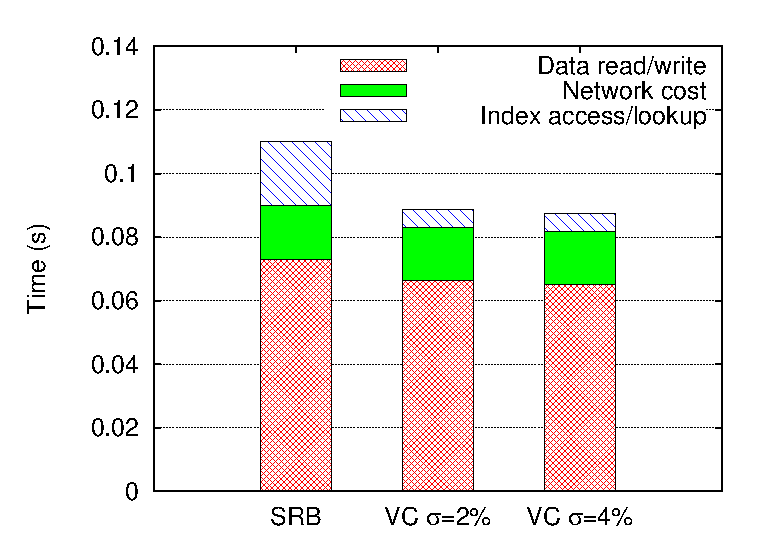
\epsfig{file=figures/vc_srb_combined, width=3in}
  \caption{Time to backup a dirty VM segment under SRB and VC appraoches}
  \label{fig:vc_srb_combined}
\end{figure}

% \begin{figure}[htbp]
%   \centering
%   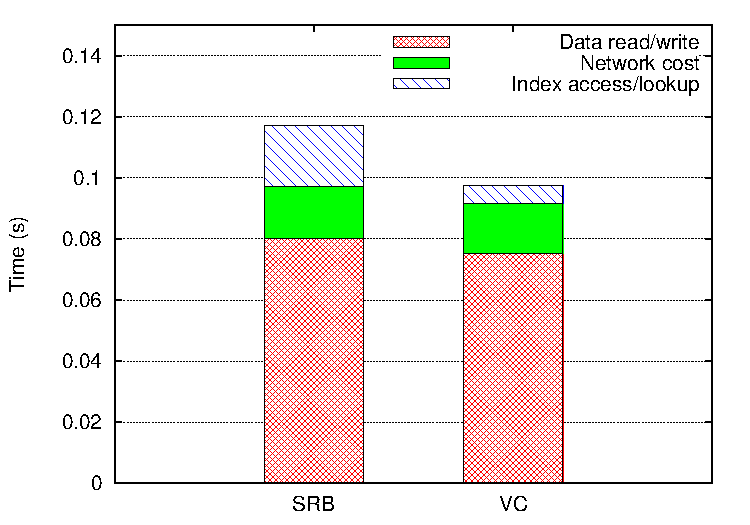
\epsfig{file=figures/srb_vs_vc, width=3in}
%   \caption{Time to backup a dirty VM segment under SRB and VC}
%   \label{fig:srb_vs_vc}
% \end{figure}

Figure~\ref{fig:vc_srb_combined} also reports the average backup time for a VM in VC when
varying the PDS size.  It lists the time distribution for data reading,
similarity-guided local search, cross-VM PDS lookup, and non-duplicate data writing. 
While data reading dominates the backup process, PDS lookup spends about a similar amount
of time as local search.
The change of $\sigma$ does not significantly affect the overall backup speed as
PDS lookup takes only a small amount of time.

% \begin{figure}
%     \centering
%     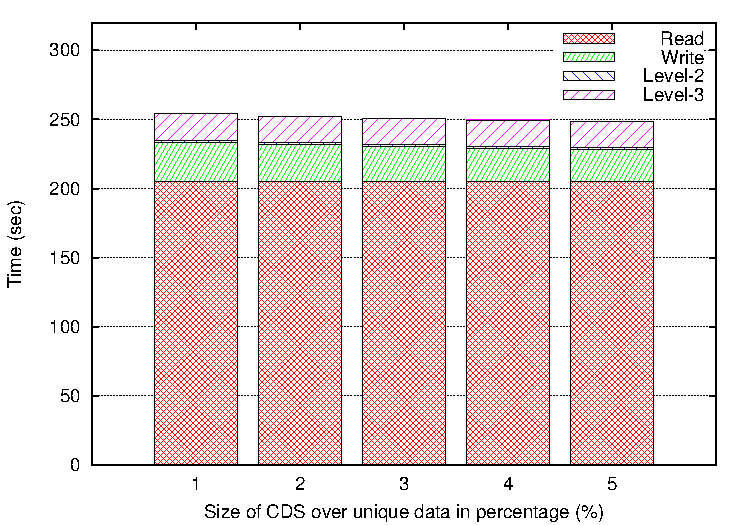
\includegraphics[width=3in]{figures/single_backup_time}
%     \caption{Average time to backup a VM in VC with varying PDS sizes}
%     \label{fig:single_vm_backup}
% \end{figure}


\begin{table*}[t]
    \centering
    \begin{tabular}{c|ccc|ccc}
    Num. of concurrent      & \multicolumn{3}{c|}{Throughput without}    & \multicolumn{3}{c}{Throughput with} \\
    backup tasks            & \multicolumn{3}{c|}{I/O throttling (MB/s)} & \multicolumn{3}{c}{I/O throttling (MB/s)} \\ \cline{2-7}
    per node                & Raw                                        & Snapshot Store & QFS  & Raw                                    & Snapshot Store & QFS  \\ \hline
    1                       & 1369.6                                     & 148.0          & 18.0 & 171.3                                  & 18.5           & 2.26 \\
    2                       & 2408.5                                     & 260.2          & 31.7 & 201.3                                  & 21.8           & 2.66 \\
    4                       & 4101.8                                     & 443.3          & 54.1 & 217.8                                  & 23.5           & 2.87 \\
    6                       & 5456.5                                     & 589.7          & 72.0 & 224.1                                  & 24.2           & 2.96 \\
    \end{tabular}
\caption{Backup throughput under different concurrency}
\label{tab:throughput}
\end{table*}
{\bf Throughput.}
Table~\ref{tab:throughput} shows the  backup throughput per each machine when all machine nodes 
handle  several VMs in parallel.
To begin, on each node we write snapshots for 4 VMs concurrently, and gradually 
increase number of VMs to 12 to saturate our system capability. We observed 
the per-node throughput peaked at 2700 MB/s when writing 10 VM snapshots in parallel, 
which is far beyond our QFS file system capability. The reason behind it is our efficient
deduplication architecture and compression which greatly reduce the amount of data that needs to be written to
the file system. The main bottleneck here is that our QFS installation only
manages one disk per node, which prevents it from fully utilizing the the
benefits of parallel disk access. We expect our architecture can
perform even better in production clusters, which often have ten or more disks on each node.


% \begin{figure}
%     \centering
%     \subfigure[Backup throughput per node under controlled I/O bandwidth usage]
%     {
%         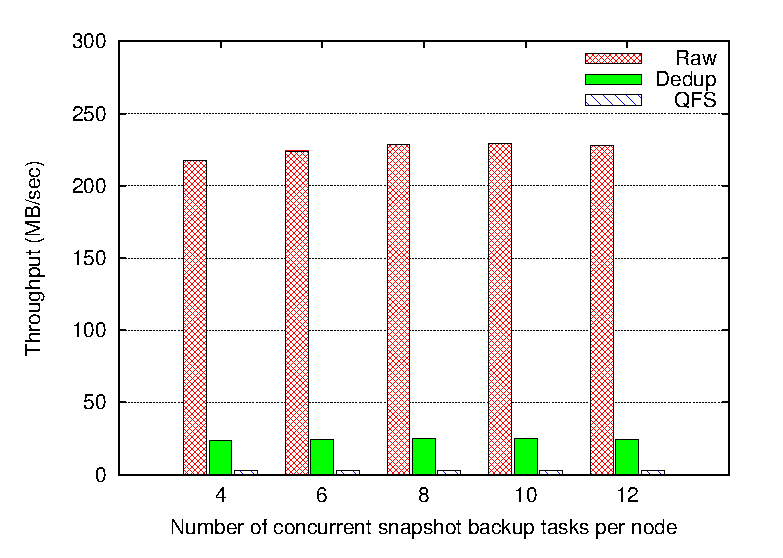
\includegraphics[width=3in]{figures/parallel_backup_with_read}
%         \label{fig:withread}
%     }
%     \\
%     \subfigure[Deduplication and storage system performance]
%     {
%         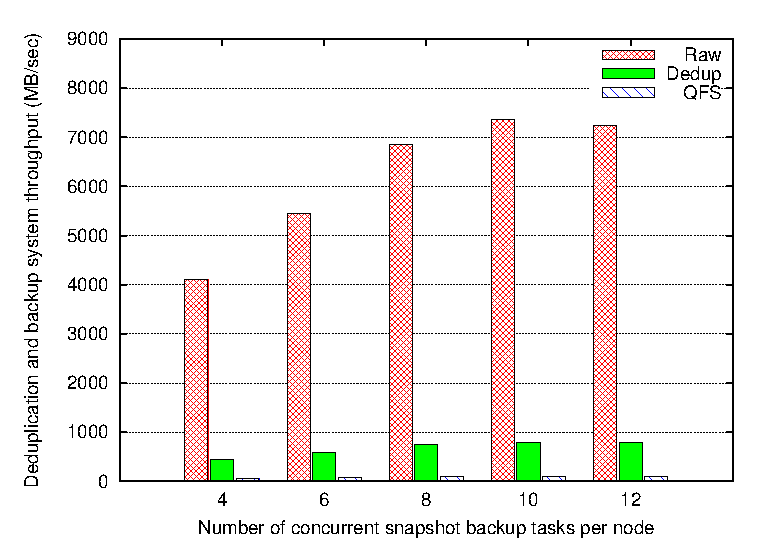
\includegraphics[width=3in]{figures/parallel_backup_no_read}
%         \label{fig:noread}
%     }
%     \caption{Throughput per-node with concurrent snapshot backup tasks}
%     \label{fig:parallel_backup}
% \end{figure}

% \subsection{Effectiveness of Approximate Deletion}
% \begin{figure}
%     \centering
%     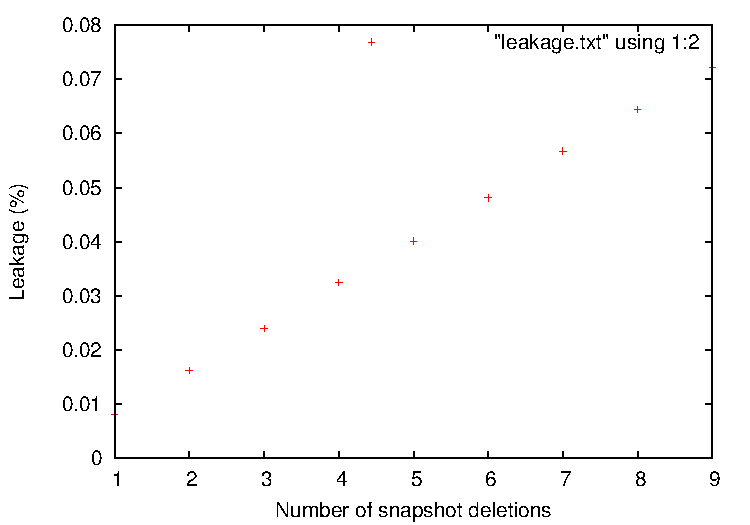
\includegraphics[width=3in]{figures/leakage}
%     \caption{Accumulated storage leakage by approximate snapshot deletions}
%     \label{fig:leakage}
% \end{figure}

Figure~\ref{fig:leakage} shows the average accumulated storage leakage in terms of percentage of
storage space per VM caused  by approximate deletions.
The solid line is the predicted leakage using Formula~\ref{eq:leakrepair} from Section~\ref{sect:delete}
while the dashed line is the actual leakage measured during the experiment.
% [OTHER PARAMETERS USED]
After 9 snapshot deletions, the actual leakage reaches 0.01\% and this means that
there is only 1MB space leaked for every 10GB of stored data. 
